%----------------------------------------------------------------------------------------
%	XieXie Programming Guide TeX File
%----------------------------------------------------------------------------------------

\documentclass{report}


%----------------------------------------------------------------------------------------
%	PACKAGES
%----------------------------------------------------------------------------------------

\usepackage{amsmath}
\usepackage{listings}
\usepackage{color}
\usepackage{pxfonts}
\usepackage{geometry}
\usepackage[T1]{fontenc}
\usepackage[ngerman, english]{babel}
\usepackage[ngerman]{hyperref}
\usepackage{xspace}
\usepackage{longtable}
\usepackage{multirow}
\usepackage{graphicx}
\usepackage{subcaption}
\usepackage{scalerel,amssymb}

\geometry{
	a4paper,
	top=20mm,
	bottom=20mm,
	margin=20mm,
}

\hypersetup{
	colorlinks = true, % Colors links instead of ugly boxes
	urlcolor = blue, % Color of external hyperlinks
	linkcolor = blue, % Color of internal links
	citecolor = blue % Color of citations
}

\definecolor{brightBlueColor}{rgb}{0.5, 0.5, 1.0}
\definecolor{darkBlueColor}{rgb}{0.0, 0.0, 0.5}
\definecolor{weakGreen}{rgb}{0.1, 0.9, 0.1}
\definecolor{weakYellow}{rgb}{0.8, 0.8, 0.1}
\definecolor{weakOrange}{rgb}{0.8, 0.5, 0.1}
\definecolor{weakRed}{rgb}{0.9, 0.1, 0.1}

\def\xiexie{\textsc{Xi\`eXie}\xspace}
\def\xxlang{\xiexie programming language\xspace}
\def\cpp{\textsc{C++}\xspace}
\def\cppx{\textsc{C++11}\xspace}
\def\java{\textsc{Java}\xspace}
\def\python{\textsc{Python}\xspace}
\def\xxc{\texttt{xxc}\xspace}
\def\xvm{\texttt{xvm}\xspace}
\def\done{\textcolor{weakGreen}{done}}
\def\almdone{\textcolor{weakYellow}{almost done}}
\def\incompl{\textcolor{weakOrange}{incomplete}}
\def\notimpl{\textcolor{weakRed}{not yet implemented}}
\def\windows{\textsc{Windows}\xspace}
\def\linux{\textsc{GNU/Linux}\xspace}

\newcommand\equalhat{%
	\let\savearraystretch\arraystretch
	\renewcommand\arraystretch{0.3}
	\begin{array}{c}
	\stretchto{
		\scalerel*[\widthof{=}]{\wedge}
		{\rule{1ex}{3ex}}%
	}{0.5ex}\\ 
	=%
	\end{array}
	\let\arraystretch\savearraystretch
}

\newcommand\SetLanguageXX{
	\lstset{
		language = C++,
		basicstyle = \footnotesize\ttfamily,
		commentstyle = \itshape\color{brightBlueColor},
		keywordstyle = \bfseries\color{darkBlueColor},
		stringstyle = \color{red},
		frame = single,
		tabsize = 4,
		numbers=none
	}
	\lstset{
		morekeywords = {
			var, super, foreach, repeat, init, release, and, or, not, null, import, module
		}
	}
}

\newcommand\SetLanguageXASM{
	\lstset{
		language = {[Motorola68k]Assembler},
		basicstyle = \footnotesize\ttfamily,
		commentstyle = \itshape\color{brightBlueColor},
		keywordstyle = \bfseries\color{darkBlueColor},
		stringstyle = \color{red},
		frame = single,
		tabsize = 4,
		numbers=left
	}
	\lstset{
		morekeywords = {
			MOV, AND, OR, XOR, SLL, SLR, ADD, SUB, MUL, DIV, MOD, ADDF, SUBF, MULF, DIVF, PUSH, POP, STOP,
			CALL, INVK, INSC, JMP, JE, JNE, JG, JL, JGE, JLE, CMP, CMPF, RET, LDB, STB, LDH, STH, LDW, STW,
			LDA, INC, DEC, NOT, ITF, FTI,
			$r0, $r1, $r2, $r3, $r4, $r5, $r6, $r7, $r8, $r9,
			$r10, $r11, $r12, $r13, $r14, $r15, $r16, $r17, $r18, $r19,
			$r20, $r21, $r22, $r23, $r24,
			$ar, $xr, $gp, $sp, $lb, $pc
		}
	}
}

\SetLanguageXX


%----------------------------------------------------------------------------------------
%	TITLE PAGE
%----------------------------------------------------------------------------------------

\newcommand*{\plogo}{\fbox{$\mathcal{LH}$}\xspace} % Generic publisher logo
\newcommand*{\titleGM}{\begingroup % Create the command for including the title page in the document
\hbox{ % Horizontal box
\hspace*{0.2\textwidth} % Whitespace to the left of the title page
\rule{1pt}{\textheight} % Vertical line
\hspace*{0.05\textwidth} % Whitespace between the vertical line and title page text
\parbox[b]{0.75\textwidth}{ % Paragraph box which restricts text to less than the width of the page

{\noindent\Huge\bfseries \xiexie Programming Guide}\\[2\baselineskip] % Title
{\large \textit{A beginner guidance for the Xi\`eXie programming language}}\\[4\baselineskip] % Tagline or further description
{\Large Lukas \textsc{Hermanns}} % Author name

\vspace{0.5\textheight} % Whitespace between the title block and the publisher
{\noindent Updated on \today}\\[\baselineskip] % Publisher and logo
}}
\endgroup}


%----------------------------------------------------------------------------------------
%	DOCUMENT INFORMATION
%----------------------------------------------------------------------------------------

%\title{\xiexie Programming Guide \\ {\normalsize Version 2.0 Alpha}}
%\author{Lukas \textsc{Hermanns}}
%\date{\today}

\begin{document}

\titleGM
%\maketitle


%----------------------------------------------------------------------------------------
%	ABOUT THE AUTHOR
%----------------------------------------------------------------------------------------

\chapter*{About the Author}

My name is Lukas Hermanns (age-group 1990) and I started this project during my studies in 2014.
By now I have over 12 years of experience in computer programming, started at the age of 12.
I have been writing programs in Basic languages such as \textsc{QBasic}, \textsc{PureBasic}, and \textsc{Blitz3D};
in high level languages such as \textsc{C}, \textsc{C++}, \textsc{C\#}, \textsc{Objective-C}, and \textsc{Java};
but also in scripting languages such as \textsc{JavaScript} and \textsc{Python}.
I'm actually a preferred programmer in C++ (meanwhile \cppx), low level stuff, and graphics programming
with shading languages such as GLSL and HLSL.

The \xxlang is intended to be simple and not tuned for performance.
It was originally designed to be used for scripting in video games, but can also be used for
general purposes.

If you like, you can follow me on \href{https://twitter.com/LukasBanana}{Twitter},
\href{https://www.youtube.com/user/SoftPixel}{YouTube}, \href{https://github.com/LukasBanana}{GitHub},
or \href{https://bitbucket.org/LukasBanana}{Bitbucket}.


%----------------------------------------------------------------------------------------
%	TODO LIST
%----------------------------------------------------------------------------------------

\chapter*{ToDo List}

The compiler, and partially the virtual machine, are not yet completed. Some rules and explanations in this report
may change over time. Here is a rough ToDo-list:

\begin{center}
\begin{tabular}[ht]{ | p{0.65 \textwidth} | p{0.25 \textwidth} | }
	\hline
	\multicolumn{2}{|c|}{\textsc{Parser}} \\
	\hline
	Implementation of parser against grammar specification & \done \\
	
	\hline \hline
	\multicolumn{2}{|c|}{\textsc{Context Analyzer}} \\
	\hline
	Expression Type Check & \done \\
	\hline
	Cast Type Check & \incompl \\
	\hline
	Automatic Type Deduction & \done \\
	\hline
	Procedure Overloading & \done \\
	\hline
	Procedure Overriding & \done \\
	\hline
	Named Parameters & \notimpl \\
	\hline
	Static and Non-Static Procedure Behavior & \incompl \\
	\hline
	Class and Procedure Attributes & \notimpl \\
	
	\hline \hline
	\multicolumn{2}{|c|}{\textsc{Code Generator}} \\
	\hline
	Common CFG and TAC Generation from DAST & \incompl \\
	\hline
	CFG Simplification & \almdone \\
	\hline
	If Statement & \done \\
	\hline
	Switch Statement & \incompl \\
	\hline
	Return Statement & \done \\
	\hline
	For Loop & \done \\
	\hline
	Range-Based For Loop & \done \\
	\hline
	Repeat Loop & \done \\
	\hline
	While Loop & \done \\
	\hline
	Do-While Loop & \done \\
	
	\hline \hline
	\multicolumn{2}{|c|}{\textsc{Optimizer}} \\
	\hline
	Constant Folding & \done \\
	\hline
	Local Constant Propagation & \almdone \\
	\hline
	Local Copy Propagation & \notimpl \\
	\hline
	Local Variable Clean & \almdone \\
	\hline
	Local Variable Reduction & \incompl \\
	
	\hline \hline
	\multicolumn{2}{|c|}{\textsc{XASM Backend}} \\
	\hline
	Final code generation for XASM & \incompl \\
	\hline
	Register Allocator & \incompl \\
	\hline
	Core Assembly File & \incompl \\
	\hline
\end{tabular}
\end{center}


\tableofcontents


%----------------------------------------------------------------------------------------
%	THE XIEXIE PROGRAMMING LANGUAGE
%----------------------------------------------------------------------------------------

\part{The \xiexie Programming Language}


%----------------------------------------------------------------------------------------
%	INTRODUCTION
%----------------------------------------------------------------------------------------

\chapter{Introduction}

First of all, ``xi\`exie'' is the chinese word for ``thanks'' or ``thank you''
(see \href{http://dictionary.hantrainerpro.com/chinese-english/translation-xiexie_thankyou.htm}{hantrainerpro.com})
and is roughly pronounced ``Sh-eh sh-eh''.

The design of the \xxlang is overall influenced by \java, \cpp, and \python.


%----------------------------------------------------------------------------------------
%	WHAT IS XIEXIE?
%----------------------------------------------------------------------------------------

\section{What is \xiexie?}

The \xiexie programming language is a high-level, object-oriented, scripting language with compiler and virtual machine.
The \xiexie compiler (XXC) translates the \xiexie code (XX) to a virtual assembler (XASM), then assembles it to
\xiexie byte code (XBC), which can then be interpreted by the \xiexie virtual machine (XVM).


%----------------------------------------------------------------------------------------
%	WHY IS IT CALLED XIEXIE?
%----------------------------------------------------------------------------------------

\section{Why is it called ``\xiexie''?}

Some years, before I started with the development of this compiler, I already had some ideas about a name for it
--- at this time the compiler was intended to be a cross compiler, i.e. to compile the \xiexie code to \cpp.
The first idea I had in mind, was to call it ``C+=2'' or ``C++++'' because it should be a more comfortable and easier
\cpp variant. But this name looked and sounded strange. Another idea was to call it ``C power of C''
(in mathematical notation $C^C$). But that still was not what I was looking for.
Then I remembered me to the Chinese word ``Xi\`exie'' which means ``Thanks'' in English and it sounds a little
similar to ``CC'' which could be seen as a shortcut for $C^C$. That's the \xiexie compiler's story about its name.

Or to make a long story short: I saw this word on a napkin in a Chinese restaurant and thought to my self: That's it! :-)


%----------------------------------------------------------------------------------------
%	MOTIVATION
%----------------------------------------------------------------------------------------

\section{Motivation}

There are many great programming languages out there. Some produce faster code than others, but some
are simpler and have a better learning curve. Using a new language doesn't mean to give up a previous one,
because every language has its own domain. For example, the performance of interpreted languages such as \python
is totally sufficient for many applications. We don't need maximal performance for a script which does some
socket connection or text processing for instance.
But I would not write the compiler and interpreter for \python in a scripted language.
There are also many ways to combine several languages: an interpreter could be used for scripting in video games
for instance. But the game engine is written in \cpp.
This is how it is done in \textsc{Unity3D} (see \href{http://www.unity3d.com/}{www.unity3d.com}).
They use \textsc{Mono} as compiler and interpreter framework for \textsc{C\#}. But the engine itself is written in \cpp.

Now \xiexie is aimed to be used for small scripting purposes, with a gentle learning curve.
The great thing about its interpreter is, that it is very tiny and can easily be integrated into
existing \textsc{C} or \cpp code. This virtual machine only consists of a single code file (written in \textsc{C99})
and can simply be included into any \textsc{C99} compliant project.


%----------------------------------------------------------------------------------------
%	SYNTAX
%----------------------------------------------------------------------------------------

\chapter{Syntax}

We start out with the syntax.


%----------------------------------------------------------------------------------------
%	BASICS
%----------------------------------------------------------------------------------------

\section{Basics}

\subsection{Commentaries}

Commentaries are a fundamental part of programming languages and they are nearly identical to those
in \java:
\begin{lstlisting}
// Single-line comment

/* Single-line comment */

/*
Multi-line comment
*/
\end{lstlisting}
Although they are very similar to the commentaries in \java, nested multi-line comments are allowed as well:
\begin{lstlisting}
/*
Outer comment
/* Nested comment */
*/
\end{lstlisting}

\subsection{Identifiers}

Identifiers (for variables, classes, etc.) must only contain alpha-numeric characters and the underscore.
They must also begin with a letter or an underscore. But there is a small exception: they must not begin with
\texttt{\_\_xx\_\_}, because all identifiers with this prefix are reserved for internal use of the compiler. \\ \\
Valid identifiers are:
\begin{itemize}
	\item \texttt{\_name\_}
	\item \texttt{FooBar}
	\item \texttt{number\_of\_wheels}
	\item \texttt{Customer01}
	\item \dots
\end{itemize}
Invalid identifiers are:
\begin{itemize}
	\item \texttt{na\"{i}ve}
	\item \texttt{Foo.Bar}
	\item \texttt{number-of-wheels}
	\item \texttt{3over2}
	\item \dots
\end{itemize}

\subsection{Literals}

These are the kinds of literals:
\begin{itemize}
	\item Boolean Literal: \texttt{true}, \texttt{false}
	\item Integer Literal (Binary): e.g. \texttt{0b11001}, \texttt{0b0000}
	\item Integer Literal (Octal): e.g. \texttt{0o24}, \texttt{0o01234567}
	\item Integer Literal (Decimal): e.g. \texttt{3}, \texttt{12}, \texttt{999}, \texttt{1234567890}
	\item Integer Literal (Hexa-Decimal): e.g. \texttt{0xff}, \texttt{0x00}, \texttt{0xaB29}
	\item Float Literal: e.g. \texttt{0.0}, \texttt{3.5}, \texttt{12.482}
	\item String Literal: e.g. \texttt{"Foo Bar"}, \texttt{"Hello, World"}, \texttt{"\textbackslash n\textbackslash t"},
		\texttt{"1st fragment"\textvisiblespace"2nd fragment}
	\item Verbatim String Literal: e.g. \texttt{@"\textbackslash home\textbackslash test"}, \texttt{@"a ""b"" c"}
\end{itemize}
Integer and float literals may optionally contain the single quotation mark as digit separator, for better readability.
If it's used, all separators must satisfy the following rules:
\begin{enumerate}
	\item For decimal literals, the separators must be \textbf{three steps apart} from each other, beginning at the dot. \\
		Example: \texttt{12'345}, \texttt{3.141'592'654}, or \texttt{-27'836.283'74}.
	\item For non-decimal literals, the separators must be \textbf{four steps apart} from each other, beginning at the dot. \\
		Example: \texttt{0xff0'214b}, \texttt{0b100'1101'1011}, \texttt{0o1234'5670}
	\item A separator must not appear at the beginning or the end of the literal. \\
		Counterexample: \texttt{'123'456'}.
	\item No valid separator must be omitted. \\
		Counterexample: \texttt{1234'567'890}.
\end{enumerate}


%----------------------------------------------------------------------------------------
%	OPERATORS
%----------------------------------------------------------------------------------------

\section{Operators}

The most operators as in \java or \cpp are also available in \xiexie:
\begin{lstlisting}
/* Arithmetic Operators */
a + b   // Addition
a - b   // Substration
a * b   // Multiplication
a / b   // Division
a % b   // Modulo
a << b  // Left Shift
a >> b  // Right Shift
-a      // Negate

/* Bitwise Operators */
a & b   // Bitwise AND
a | b   // Bitwise OR
a ^ b   // Bitwise XOR
~a      // Bitwise NOT

/* Boolean Operators */
not a   // Logic NOT
a and b // Logic AND
a or b  // Logic OR

/* Relation Operators */
a = b   // Equality
a != b  // Inequality
a < b   // Less
a <= b  // Less Or Equal
a > b   // Greater
a >= b  // Greater Or Equal
\end{lstlisting}
As the interested reader may have noticed, the \textit{equality operator} is different to that in the most languages.
This is because the \textit{copy assignment} operators is \texttt{:=} and not \texttt{=}.
\begin{lstlisting}
x := 5       // ok, set x to 5
a, b, c := 4 // ok, set a, b, and c to 4
a := b := 3  // error, b := 3 is not an expression
\end{lstlisting}
In the above example \texttt{a := b := 3} is invalid, because on the right hand side of the first \texttt{:=} must be
an expression. But per definition in \xiexie \texttt{b := 3} is not an expression, but a statement!
The variable list assignment (\texttt{a, b, c := \dots}) is a comfort functionality, which is only supported for the
copy assignment.

The modify-assign operators are available as well:
\begin{lstlisting}
a += b
a -= b
a *= b
a /= b
a %= b
a <<= b
a >>= b
a &= b
a |= b
a ^= b
\end{lstlisting}
However, they are also not allowed inside another expression.


%----------------------------------------------------------------------------------------
%	TYPE DENOTERS
%----------------------------------------------------------------------------------------

\section{Type Denoters}

\subsection{Built-in Types}

There are only the following three built-in data types:
\begin{lstlisting}
bool  // Boolean type; can be `true' or `false'
int   // 32-bit signed integral type
float // 32-bit floating-point type
\end{lstlisting}

\subsection{Objects}

%There are two kinds of objects.
Types for class objects (more about classes in chapter \ref{ch:classes}) are written as follows:
\begin{lstlisting}
// Empty string
String s

// List of strings
String s1 := "Hello, World", s2 := "Foo", s3 := "Bar"
\end{lstlisting}

\subsection{Arrays}

The only generic way for lists are the built-in arrays:
\begin{lstlisting}
// Declare array objects with initializer lists
int[] intArray := { 1, 2, 3 }
float[][] floatArrayArray := { { 0.0, 1.5 }, { 3.5, 1.23 } }
String[] stringArray := { "a", "b", "c" }

// Access array elements
String s1 := stringArray[0]
String s2 := stringArray[intArray[0]]
float[] floatArray := floatArrayArray[1]
\end{lstlisting}

\subsection{Automatic Type Deduction}

Whereas automatic type deduction in \cppx is a very extensive language feature,
in \xiexie it can be summarized in this section.
There are two keywords for automatic type deduction: \texttt{var} and \texttt{const}. As the name implies
\texttt{var} denotes a variable type and \texttt{const} denotes a constant type. The latter type is the only way
to define constants in \xiexie. Here are a few examples:
\begin{lstlisting}
var   i  := 1       // i is from type 'int'
var   f  := 3.5     // f is from type 'float'
var   s  := "."     // s is from type 'String'
var   a  := { 5 }   // a is from type 'array of int'
var   aa := {       // aa is from type 'array of array of String'
  { "test" },
  { "a", "b" }
}

const ci := 5       // ci is a constnat int with value 5
const cj := ci*2    // cj is a constant int with value 10
const cf := 3.14    // cf is a constant float
const cb := ci > cj // cb is a constant bool with value 'false'
\end{lstlisting}


%----------------------------------------------------------------------------------------
%	STATEMENTS
%----------------------------------------------------------------------------------------

\section{Statements}

Unlike \cpp and \java, there are no semicolons in \xiexie to terminate statements.
Only the regular \texttt{for}-statement has two semicolons, to separate the initializer statement,
the conidition expression, and the increment statement. This means the compiler
(or rather the \textit{parser}, which reads the source code) always knows when a statement or expression is complete.
But it also means that you --- the programmer --- can do weird things with this syntax. Consider the following code sample:
\begin{lstlisting}
int a:=3
-4
,b:=-
5+2 int c
\end{lstlisting}
This is valid \xiexie code and it contains only two statements!
If we write it in a more common convention, it may look like this:
\begin{lstlisting}
int a := 3-4,
    b := -5+2
int c
\end{lstlisting}
Hence, the readability of your code is up to you and your programming style :-). The only language I've worked with,
which forces you to practice better readability is \python.
Actually a great principle, but with \xiexie you have complete freedom.

The absence of statement terminators is the reason for the \textit{double paren} syntax of attributes:
\begin{lstlisting}
[[attribute]]
\end{lstlisting}
To understand why this is the case, let's assume attributes are written with a single paren and consider
the following class declaration:
\begin{lstlisting}
class Widget {
    const c := 0 // Initialize member constant 'c' with 0
    int   v := c // Initialize member variable 'v' with constant 'c'
    [entry]      // Mark next procedure as the main entry point with attribute 'entry'
    static void main() {}
}
\end{lstlisting}
Now this doesn't seem very complex. But the parser runs into trouble when reading \texttt{[entry]}.
This is because the parser reads it as follows:
\begin{lstlisting}
int v := c[entry]
\end{lstlisting}
But \texttt{c} is not an array. This is why attributes are written with a double paren, because array accesses
never begin with '[['. They may end with ']]', but this is not important for the parser.

\subsection{Loop Statements}

It follows several examples of loop statements.

\subsubsection{\texttt{for} Loop}

\begin{lstlisting}
// This regular for loop iterates 'i' from 0 to 9 (similar to Java)
for int i := 0 ; i < 10 ; i++ {
    // Infinite loop (also similar to Java)
    for ;; {
        if i >= 0 {
            // Break infinite loop
            break
        }
    }
    
    // Inner iteration variable 'j' is implicit initialized to 0.0
    float j
    for ; j < 3.5 ; {
        j += 0.5
    }
}
\end{lstlisting}

\subsubsection{Ranged Based \texttt{for} Loop}

\begin{lstlisting}
// Print numbers 0, 1, 2, 3, and 4
for i : 0 .. 4 {
    // Print value of 'i' (this 'i' is not mutable!)
    print(i)
}

// Print numbers 10, 7, 4, 1, -2, -5, and -8
for i : 10 .. -10 -> 3 {
    print(i)
}
\end{lstlisting}

\subsubsection{\texttt{foreach} Loop}

\begin{lstlisting}
// Iterate over array with elements 1, 2, and 3
foreach i : { 1, 2, 3 } {
    print(i)
}

// Iterate over a 'superList' from type (array of arrays of strings)
String[][] superList := { { "a", "b" }, { "c" } }
foreach list : superList {
    // Iterate over all elements in the current sub list
    foreach str : list {
        // Do something with this string
        print(str)
    }
}
\end{lstlisting}

\subsubsection{\texttt{repeat} Loop}

\begin{lstlisting}
// Repeat for unconditional iterations
// (This is internally a "ForEver"-loop)
repeat {
    // Condition to break the loop
    if magicFunction() {
        // Break loop
        break
    }
}

// Do something 10 times (with invisible index variable)
// (This is internally a "ForRange"-loop)
repeat 10 {
    doSomething()
}
\end{lstlisting}

\subsubsection{\texttt{while} Loop}

\begin{lstlisting}
// Regular while loop
while magicFunction() {
    doSomething()
}
\end{lstlisting}

\subsubsection{\texttt{do}/\texttt{while} Loop}

\begin{lstlisting}
// Regular do-while loop
do {
    doSomething()
} while magicFunction()
\end{lstlisting}


%----------------------------------------------------------------------------------------
%	EXPRESSIONS
%----------------------------------------------------------------------------------------

\section{Expressions}

\subsection{Macros}

\xiexie does not support the declaration of macros. However, there are a few built-in macros, which represent additional
reserved identifiers:
\begin{itemize}
	\item \texttt{\_\_FILE\_\_} String which contains the current filename.
	\item \texttt{\_\_CLASS\_\_} String which contains the current class name.
	\item \texttt{\_\_PROC\_\_} String which contains the current procedure name.
	\item \texttt{\_\_LINE\_\_} String which contains the current line number.
	\item \texttt{\_\_DATE\_\_} String which contains the current date and time.
\end{itemize}



%----------------------------------------------------------------------------------------
%	CLASSES
%----------------------------------------------------------------------------------------

\chapter{Classes}
\label{ch:classes}

A \xiexie program can only consist of imports, modules, and class declarations. And classes can only be defined
in the global scope. That means every procedure must be defined inside a class and inner classes are currently not supported.


%----------------------------------------------------------------------------------------
%	GETTING STARTED
%----------------------------------------------------------------------------------------

\section{Getting Started}

To get started, take a look at the following example program which prints the classical phrase ``Hello, World!''
onto the standard output:
\begin{lstlisting}[numbers=left]
// XieXie Hello World Program
import System
class HelloWorld {
    static void main() {
        System.out.writeLine("Hello, World!")
    }
}
\end{lstlisting}
This merely writes the line ``\texttt{Hello, World!}'' to the standard output. Let's take a closer look at each line.

Line 2 imports the ``System.xx'' file from the \xiexie standard library:
\begin{lstlisting}
import System      // either this ...
import "System.xx" // ... or this
\end{lstlisting}
If the imported file is in another directory, the string version of \texttt{import} is the only choice.
This can also be omitted if the file is added to the compilation process.
The files for the classes \texttt{Object}, \texttt{String}, \texttt{Array}, and \texttt{Intrinsics}
are always implicit imported, because they are `internal' classes the compiler knows generally.
Note that verbatim strings are allowed wherever string literals are allowed, i.e. the following example is valid \xiexie code:
\begin{lstlisting}
import "C:\\Program Files\\Test1.xx" // either this ...
import @"C:\Program Files\Test1.xx"  // ... or this
\end{lstlisting}
The \texttt{import} keyword is different to that in \java and also different to the \texttt{\#include} directive in \cpp.
Although it takes a filename as parameter (like \cpp's \texttt{\#include}), it does not \textit{include} the file in place.
Whenever an \texttt{import} is read by the \textit{parser}, the filename is added to the set of import files.
After all source files have been read, which were passed as input to the compiler, all import files will be read next.
This will be repeated until no new files are added to the set.
Consider this is a \textit{set} of files, i.e. several \texttt{import} commands may occur with the same filename,
but it will be read only once. This is why the above sample is valid \xiexie code. It also means that recursive imports
are allowed as well:
\begin{lstlisting}
// File1.xx
import "File2.xx"
\end{lstlisting}
\begin{lstlisting}
// File2.xx
import "File1.xx"
\end{lstlisting}

Line 3 declares the class \texttt{HelloWorld} which implicit inherits from the base class \texttt{Object},
like it is done in \java:
\begin{lstlisting}[numbers=left, firstnumber=3]
class HelloWorld { /* ... */ }
\end{lstlisting}
To inherit from other classes, just write a colon and the identifier of the base class:
\begin{lstlisting}
class SubClass : BaseClass { /* ... */ }
\end{lstlisting}
There is no multiple inheritance like in \cpp or interfaces like in \java!

The next line declares the procedure \texttt{main}.
\begin{lstlisting}[numbers=left, firstnumber=4]
static void main() {
\end{lstlisting}
This is the main entry point for the program. There can only be one main entry point, but there are several possible
signatures for this procedure:
\begin{lstlisting}
// No return value, no arguments
static void main() { /* ... */ }

// No return value, arguments
static void main(String[] args) { /* ... */ }

// Return value, no arguments
static int main() { /* ... */ }

// Return value, arguments
static int main(String[] args) { /* ... */ }
\end{lstlisting}

The last line of code prints the message to the standard output:
\begin{lstlisting}[numbers=left, firstnumber=5]
System.out.writeLine("Hello, World!")
\end{lstlisting}
\texttt{System} is a class from the standard \xiexie library, \texttt{out} is a \textit{static} member
from the type 'OutputStream', and \texttt{writeLine} is a function which takes a string as input.


%----------------------------------------------------------------------------------------
%	DECLARATION RULES FOR CLASSES
%----------------------------------------------------------------------------------------

\section{Declaration Rules for Classes}

In \xiexie there is no need for \textit{forward declarations}. Everything can be declared in the respective scope
and is accessible throughout the entire program (except private scope). This is why the following code is valid:
\begin{lstlisting}
// First declare sub class
class SubClass : BaseClass { /* ... */ }

// Then declare base class
class BaseClass { /* ... */ }
\end{lstlisting}
The same applies for procedure declarations:
\begin{lstlisting}
class B {
    static void procB1() {
        A.procA()  // no forward declaration required ...
        B.procB2() // ... same here
    }
    static void procB2() { /* ... */ }
}
class A {
    static void procA() { /* ... */ }
}
\end{lstlisting}
This works because the \textit{context analyzer} of the compiler works in several phases:
\begin{enumerate}
	\item Class symbols are registered in global scope.
	\item Class signatures are analyzed (attributes and base class).
	\item Class inheritance is verified (check for cycles).
	\item Class member symbols are registred in respective class scope (procedures, variables, etc.).
	\item Procedure code is analyzed.
\end{enumerate}


%----------------------------------------------------------------------------------------
%	PROCEDURES
%----------------------------------------------------------------------------------------

\section{Procedures}

In \xiexie we talk about \textit{procedures} (somethings called \textit{methods}),
because in the strict sense \textit{functions} have no side effects.
Functions have only input parameters which are calculated to a result. But in \xiexie every procedure can have side effects,
meaning that they can modify the program state (with static variables for instance).

\subsection{Procedure Signature}

A \textit{procedure signature} is the extended identification of a procedure beyond its identifier string.
The signature consists of the identifier string, its parameter list, and the procedure's return type.
However, the return type is never used for identification.

\subsection{Procedure Overloading}

\xiexie supports overloading of procedures. This means the same identifier can be used several times
for procedures inside a class declaration (including its inheritance hierarchy).
This requires that the following rules are satisfied:
\begin{quote}
	All procedures with the same identifier inside a class declaration can be distinguished by their
	parameter count or parameter types.
\end{quote}
Here is an example of procedure overloading.
\begin{lstlisting}
class Widget {
    int f() {
        return 1
    }
    int f(int x) {
        return x*2
    }
    float f(float x) {
        return x*3.0
    }
    void caller() {
        int   a := f()    // a is 1
        int   b := f(1)   // b is 2
        float c := f(2.0) // c is 6.0
    }
}
\end{lstlisting}
When overloading procedures, try to avoid ambiguities with default arguments. Adding default arguments
to all parameters of all overloaded procedures is allowed, but procedure calls may be ambiguous for the compiler:
\begin{lstlisting}
class Widget {
    int f() { /* ... */ }
    int f(int x := 0) { /* ... */ }
    float f(float x := 0.0) { /* ... */ }
    
    void caller() {
        int   a := f()    // error, could be f(), f(int x := 0), or f(float x := 0.0)
        int   b := f(1)   // ok, argument is from type 'int'
        float c := f(2.0) // ok, argument is from type 'float'
    }
}
\end{lstlisting}

\subsection{Procedure Overriding}

\xiexie supports overriding of procedures. This means the same procedure signature can be used inside a class and its
base class. The procedure calls of overloaded and overridden procedures require that the following rules are satisfied:
\begin{quote}
	If a procedure with identifier $P$ is declared inside a class $C$, a procedure with the same identifier is declared
	in its base class $B$ but with another signature, and another procedure inside class $C$ calls the procedure $P$
	from class $B$, then the identifier \texttt{super} must be specified in front of the call.
\end{quote}
To better understand this awkward definition, take a look at this example:
\begin{lstlisting}
class B {
    int f(int x, int y) {
        return 1
    }
    int g() {
        return 2
    }
}
class S : B {
    int f(int x) {
        return 3
    }
    void caller() {
        int a := f(0)          // equivalent to 'this.f(0)'
        int b := super.f(0, 0) // 'super' is required, due to overloaded procedure 'f'
        int c := g()           // no need for 'super', because 'g' is not overloaded
    }
}
\end{lstlisting}


%----------------------------------------------------------------------------------------
%	ATTRIBUTES
%----------------------------------------------------------------------------------------

\section{Attributes}

There are several attributes for class-, procedure-, and variable declarations:
\begin{lstlisting}
// Class A is marked as 'deprecated'.
[[deprecated]]
class A {
    // Declare some procedure
    void p() {}
}

// Class B is marked as 'deprecated' with a hint.
// Since B is deprecated as well, the deprecation of A is ignored here.
[[deprecated("hint...")]]
class B {
    // Mark 'p' to override 'A.p'. If 'p' does not match the signature
    // of procedure 'A.p', the compiler will throw an error message.
    [[override]]
    void p() {}
}

// Class C is 'final', i.e. no class can inherit from C.
// Because A is deprecated but not C, the compiler will throw a warning.
[[final]]
class C : A {}
\end{lstlisting}
Here is a summary of all attributes:
\begin{itemize}
	\item \textbf{\texttt{deprecated}}, \textbf{\texttt{deprecated(String)}}
		Marks a class, procedure, or member-variable as deprecated.
	\item \textbf{\texttt{override}} Overrides a procedure from a class in its inheritance hierarchy.
	\item \textbf{\texttt{final}} Makes a class final, which disables to inherit from this class.
\end{itemize}


%----------------------------------------------------------------------------------------
%	MODULES
%----------------------------------------------------------------------------------------

\chapter{Modules}
\label{ch:modules}

A \textit{module} consists of a shared library (\texttt{*.dll} on \windows and \texttt{*.so} on \linux)
and a \xiexie module file. They are similar to \python modules.


%----------------------------------------------------------------------------------------
%	USING MODULES
%----------------------------------------------------------------------------------------

\section{Using Modules}

Module declarations are similar to external classes. But they can only have static procedures. Here is an example:
\begin{lstlisting}
module MyModule {
    static void doSomething(int x)
}
\end{lstlisting}
Using this in your \xiexie code will then look like this:
\begin{lstlisting}
import MyModule
class MyClass {
    static void main() {
        MyModule.doSomething(42)
    }
}
\end{lstlisting}


%----------------------------------------------------------------------------------------
%	Creating MODULES
%----------------------------------------------------------------------------------------

\section{Creating Modules}

Modules must be written in plain C or \cpp. A minimal module would consist of three files.
Supposed our example module is named ``MyModule'' and we work on \windows we would have these files:
\begin{itemize}
	\item \textbf{\texttt{MyModule.c}} Module code written in C.
	\item \textbf{\texttt{MyModule.dll}}/ \textbf{\texttt{.so}} Shared library which runs the module code.
	\item \textbf{\texttt{MyModule.xx}} \xiexie code file which declares the module. 
\end{itemize}
The C code file must implement the following function interfaces to be a valid \xiexie module:
\begin{lstlisting}
// Returns the number of module procedures.
int xx_module_proc_count();

// Returns the procedure for the respective index.
XVM_INVOCATION_PROC xx_module_fetch_proc(int index);

// Returns the procedure identifier for the respective index.
const char* xx_module_fetch_ident(int index);
\end{lstlisting}
Our simple module example from above could be implemented as follows:
\begin{lstlisting}
#include "../xx_module.h"

// This is our module procedure "soSomething".
// All module procedures must have this interface.
void doSomething(xvm_env env) {
    // Get 1st parameter from XVM environment
    int x = xvm_param_int(env, 1);
    
    // Do something with 'x'
    printf("input parameter 'x' is %i\n", i);
    
    // Pop arguments from stack (1 for the single parameter 'x')
    xvm_return_void(env, 1);
}

// Implement the module interface
static xvm_invocation procList[] = {
    { "doSomething", doSomething },
};

XVM_IMPLEMENT_MODULE_INTERFACE(procList);
\end{lstlisting}


%----------------------------------------------------------------------------------------
%	DEVELOPER TOOLS
%----------------------------------------------------------------------------------------

\part{Developer Tools}


%----------------------------------------------------------------------------------------
%	COMPILER
%----------------------------------------------------------------------------------------

\chapter{Compiler}


%----------------------------------------------------------------------------------------
%	COMMAND LINE TOOL
%----------------------------------------------------------------------------------------

\section{Command Line Tool}

The compiler can be used as command line tool. The appropriate program is named \xxc.
Enter \texttt{xxc help} in a command line to see the manual pages.

In contrast to most other command line tools, the commands for \xxc don't have the `-' prefix.
Instead the command options use this prefix. Here is an example:
\begin{quote}
\texttt{xxc C -f FILE1 -f FILE2 -O}
\end{quote}
The above command line uses the \texttt{C} command (also \texttt{compile}) with the flags `-f' and `-O'.

\subsection{Output}

The compiler tries to show you where an error or warning occurred.
If possible, it is highlighted with a \textit{line marker}. Consider the following code sample:
\begin{lstlisting}
class Foo {
    void Bar() {
        int x := y
    }
}
\end{lstlisting}
Now consider the compiler processes this code with the following command line:
\begin{quote}
\texttt{xxc C -f Core.xx -f Foo.xx}
\end{quote}
Then the compiler indicates that the variable 'y' was not declared (see Figure \ref{fig:compiler-output}).
\begin{figure}[ht]
	\centering
	\begin{subfigure}[here]{0.9 \textwidth}
		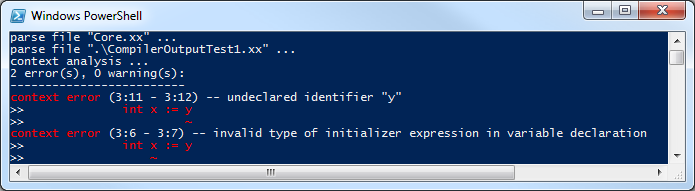
\includegraphics[width=\textwidth]{images/compiler-output-win32}
		\caption{Output in \textsc{PowerShell} on \windows 7}
		\label{fig:compiler-output-win32}
	\end{subfigure}
	\begin{subfigure}[here]{0.9 \textwidth}
		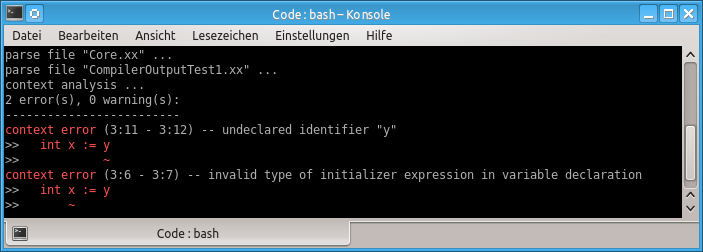
\includegraphics[width=\textwidth]{images/compiler-output-linux}
		\caption{Output in \textsc{Terminal} on \textsc{Kubuntu} \linux}
		\label{fig:compiler-output-linux}
	\end{subfigure}
	\caption{Compiler output for the above code sample.}
	\label{fig:compiler-output}
\end{figure}
As you can see, some errors may produce multiple outputs. In this case, 'y' is undeclared which produces two error
outputs here:
\begin{enumerate}
	\item The identifier 'y' is undeclared, so the appearance in the initializer expression is invalid.
	\item The type of the initializer expression for the declaration of 'x' can not be deduced, so the type check fails.
\end{enumerate}


%----------------------------------------------------------------------------------------
%	VIRTUAL MACHINE
%----------------------------------------------------------------------------------------

\chapter{Virtual Machine}

The \textsc{\xiexie Virtual Machine} (XVM) is a separated program (named \xvm), written in pure C99.


%----------------------------------------------------------------------------------------
%	EXECUTING PROGRAMS
%----------------------------------------------------------------------------------------

\section{Executing Programs}

To execute (or run) a virtual program, just enter the filename of an \texttt{*.xbc} file into the \xvm:
\begin{quote}
\texttt{xvm HelloWorld.xbc}
\end{quote}


%----------------------------------------------------------------------------------------
%	LOW-LEVEL
%----------------------------------------------------------------------------------------

\part{Low-Level Programming}


%----------------------------------------------------------------------------------------
%	VIRTUAL ASSEMBLER
%----------------------------------------------------------------------------------------

\chapter{Virtual Assembler}

The \xiexie Virtual Assembler (XASM) is the low level language which is used as interface to the \xvm.
It's a very low level language, with similarities to ARM$^\text{\scriptsize\textregistered}$ Assembler.


%----------------------------------------------------------------------------------------
%	INSTRUCTION SET
%----------------------------------------------------------------------------------------

\section{Instruction Set}

\subsection{Registers}

The \xvm is a register machine, i.e. it uses registers as operands for its instructions instead of the stack.
This commonly increases performance but is a little more tricky to use, when you run out of registers.
Each register index inside an instruction is stored with 4 bits, thus there are 16 registers and this is the list:
{\small
\begin{enumerate}
	\item \textbf{\texttt{\$r0}} \xspace General Purpose Register 0. \\ \vdots
	\addtocounter{enumi}{23}
	\item \textbf{\texttt{\$r24}} \xspace General Purpose Register 24.
	\item \textbf{\texttt{\$ar}} \xspace Argument Return.
	\item \textbf{\texttt{\$xr}} \xspace Extended Register.
	\item \textbf{\texttt{\$gp}} \xspace Global Pointer.
	\item \textbf{\texttt{\$cf}} \xspace Conditional Flag.
	\item \textbf{\texttt{\$lb}} \xspace Local Base Pointer.
	\item \textbf{\texttt{\$sp}} \xspace Stack Pointer.
	\item \textbf{\texttt{\$pc}} \xspace Program Counter.
\end{enumerate}
}
All pointer registers and the program counter (i.e. \texttt{\$gp}, \texttt{\$lb}, \texttt{\$sp}, and \texttt{\$pc})
are all `real' pointers to the memory in your operating system. 

\subsection{OpCodes}

Each instruction stores its mnemonic (Greek `memory'$\equalhat$instruction identifier) in the first 6 bits.
This provides a maximum of 64 instructions. However, only 52 mnemonics are currently in use.

{\footnotesize
\begin{center}
\begin{tabular}[ht]{
	| p{0.07 \textwidth} | p{0.1 \textwidth} | p{0.08 \textwidth} | p{0.08 \textwidth}
	| p{0.08 \textwidth} | p{0.185 \textwidth} | p{0.2 \textwidth} |
}
	\hline
	\multicolumn{7}{|c|}{\texttt{3-Register Instruction OpCodes (00....)}} \\
	\hline \hline
	
	\multirow{2}{*}{\texttt{Mnemonic}} & \texttt{OpCode} & \texttt{Dest.} & \texttt{LSource} & \texttt{RSource} &
		\texttt{Unused} & \multirow{2}{*}{\texttt{Description}} \\
	& \texttt{31.......26} & \texttt{25.....21} & \texttt{20.....16} & \texttt{15.....11} &
		\texttt{10..................0} & \\
	\hline
	
	\texttt{AND} & \texttt{0 0 0 0 0 1} & \texttt{D D D D D} & \texttt{L L L L L} & \texttt{R R R R R} &
		\texttt{0 0 0 0 0 0 0 0 0 0 0} & Bitwise AND (D := L \& R). \\
	\hline
	
	\texttt{OR} & \texttt{0 0 0 0 1 0} & \texttt{D D D D D} & \texttt{L L L L L} & \texttt{R R R R R} &
		\texttt{0 0 0 0 0 0 0 0 0 0 0} & Bitwise OR (D := L | R). \\
	\hline
	
	\texttt{XOR} & \texttt{0 0 0 0 1 1} & \texttt{D D D D D} & \texttt{L L L L L} & \texttt{R R R R R} &
		\texttt{0 0 0 0 0 0 0 0 0 0 0} & Bitwise XOR (D := L ${\mathchar"5E}$ R). \\
	\hline
	
	\texttt{ADD} & \texttt{0 0 0 1 0 0} & \texttt{D D D D D} & \texttt{L L L L L} & \texttt{R R R R R} &
		\texttt{0 0 0 0 0 0 0 0 0 0 0} & Integer add. (D := L + R). \\
	\hline
	
	\texttt{SUB} & \texttt{0 0 0 1 0 1} & \texttt{D D D D D} & \texttt{L L L L L} & \texttt{R R R R R} &
		\texttt{0 0 0 0 0 0 0 0 0 0 0} & Integer sub. (D := L - R). \\
	\hline
	
	\texttt{MUL} & \texttt{0 0 0 1 1 0} & \texttt{D D D D D} & \texttt{L L L L L} & \texttt{R R R R R} &
		\texttt{0 0 0 0 0 0 0 0 0 0 0} & Integer mul. (D := L $\times$ R). \\
	\hline
	
	\texttt{DIV} & \texttt{0 0 0 1 1 1} & \texttt{D D D D D} & \texttt{L L L L L} & \texttt{R R R R R} &
		\texttt{0 0 0 0 0 0 0 0 0 0 0} & Integer div. (D := L $\div$ R). \\
	\hline
	
	\texttt{MOD} & \texttt{0 0 1 0 0 0} & \texttt{D D D D D} & \texttt{L L L L L} & \texttt{R R R R R} &
		\texttt{0 0 0 0 0 0 0 0 0 0 0} & Modulo (D := L \% R). \\
	\hline
	
	\texttt{SLL} & \texttt{0 0 1 0 0 1} & \texttt{D D D D D} & \texttt{L L L L L} & \texttt{R R R R R} &
		\texttt{0 0 0 0 0 0 0 0 0 0 0} & Shift left (D := L << R). \\
	\hline
	
	\texttt{SLR} & \texttt{0 0 1 0 1 0} & \texttt{D D D D D} & \texttt{L L L L L} & \texttt{R R R R R} &
		\texttt{0 0 0 0 0 0 0 0 0 0 0} & Shift right (D := L >> R). \\
	\hline
	
	\texttt{ADDF} & \texttt{0 0 1 0 1 1} & \texttt{D D D D D} & \texttt{L L L L L} & \texttt{R R R R R} &
		\texttt{0 0 0 0 0 0 0 0 0 0 0} & Float add. (D := L + R). \\
	\hline
	
	\texttt{SUBF} & \texttt{0 0 1 1 0 0} & \texttt{D D D D D} & \texttt{L L L L L} & \texttt{R R R R R} &
		\texttt{0 0 0 0 0 0 0 0 0 0 0} & Float sub. (D := L - R). \\
	\hline
	
	\texttt{MULF} & \texttt{0 0 1 1 0 1} & \texttt{D D D D D} & \texttt{L L L L L} & \texttt{R R R R R} &
		\texttt{0 0 0 0 0 0 0 0 0 0 0} & Float mul. (D := L $\times$ R). \\
	\hline
	
	\texttt{DIVF} & \texttt{0 0 1 1 1 0} & \texttt{D D D D D} & \texttt{L L L L L} & \texttt{R R R R R} &
		\texttt{0 0 0 0 0 0 0 0 0 0 0} & Float div. (D := L $\div$ R). \\
	\hline
\end{tabular}
\end{center}
}

{\footnotesize
\begin{center}
\begin{tabular}[ht]{
	| p{0.07 \textwidth} | p{0.1 \textwidth} | p{0.08 \textwidth} | p{0.08 \textwidth}
	| p{0.27 \textwidth} | p{0.22 \textwidth} |
}
	\hline
	\multicolumn{6}{|c|}{\texttt{2-Register Instruction OpCodes (01....)}} \\
	\hline \hline
	
	\multirow{2}{*}{\texttt{Mnemonic}} & \texttt{OpCode} & \texttt{Dest.} & \texttt{Source} &
		\texttt{Unused or Value} & \multirow{2}{*}{\texttt{Description}} \\
	& \texttt{31.......26} & \texttt{25.....21} & \texttt{20.....16} & \texttt{15............................0} & \\
	\hline
	
	\texttt{MOV} & \texttt{0 1 0 0 0 0} & \texttt{D D D D D} & \texttt{S S S S S} &
		\texttt{0 0 0 0 0 0 0 0 0 0 0 0 0 0 0 0} & Move (D := S). \\
	\hline
	
	\texttt{NOT} & \texttt{0 1 0 0 0 1} & \texttt{D D D D D} & \texttt{S S S S S} &
		\texttt{0 0 0 0 0 0 0 0 0 0 0 0 0 0 0 0} & Bitwise NOT (D := \textasciitilde S). \\
	\hline
	
	\texttt{FTI} & \texttt{0 1 0 0 1 0} & \texttt{D D D D D} & \texttt{S S S S S} &
		\texttt{0 0 0 0 0 0 0 0 0 0 0 0 0 0 0 0} & Float to integer (D := (int)S). \\
	\hline
	
	\texttt{ITF} & \texttt{0 1 0 0 1 1} & \texttt{D D D D D} & \texttt{S S S S S} &
		\texttt{0 0 0 0 0 0 0 0 0 0 0 0 0 0 0 0} & Integer to float (D := (float)S). \\
	\hline
	
	\texttt{AND} & \texttt{0 1 0 1 0 0} & \texttt{D D D D D} & \texttt{S S S S S} &
		\texttt{V V V V V V V V V V V V V V V V} & Bitwise AND (D := S \& V). \\
	\hline
	
	\texttt{OR} & \texttt{0 1 0 1 0 1} & \texttt{D D D D D} & \texttt{S S S S S} &
		\texttt{V V V V V V V V V V V V V V V V} & Bitwise OR (D := S | V). \\
	\hline
	
	\texttt{XOR} & \texttt{0 1 0 1 1 0} & \texttt{D D D D D} & \texttt{S S S S S} &
		\texttt{V V V V V V V V V V V V V V V V} & Bitwise XOR (D := S ${\mathchar"5E}$ V). \\
	\hline
	
	\texttt{ADD} & \texttt{0 1 0 1 1 1} & \texttt{D D D D D} & \texttt{S S S S S} &
		\texttt{V V V V V V V V V V V V V V V V} & Modulo (D := S \% V). \\
	\hline
	
	\texttt{SUB} & \texttt{0 1 1 0 0 0} & \texttt{D D D D D} & \texttt{S S S S S} &
		\texttt{V V V V V V V V V V V V V V V V} & Shift left (D := S << V). \\
	\hline
	
	\texttt{MUL} & \texttt{0 1 1 0 0 1} & \texttt{D D D D D} & \texttt{S S S S S} &
		\texttt{V V V V V V V V V V V V V V V V} & Shift right (D := S >> V). \\
	\hline
	
	\texttt{DIV} & \texttt{0 1 1 0 1 0} & \texttt{D D D D D} & \texttt{S S S S S} &
		\texttt{V V V V V V V V V V V V V V V V} & Integer add. (D := S + V). \\
	\hline
	
	\texttt{MOD} & \texttt{0 1 1 0 1 1} & \texttt{D D D D D} & \texttt{S S S S S} &
		\texttt{V V V V V V V V V V V V V V V V} & Integer sub. (D := S - V). \\
	\hline
	
	\texttt{SLL} & \texttt{0 1 1 1 0 0} & \texttt{D D D D D} & \texttt{S S S S S} &
		\texttt{V V V V V V V V V V V V V V V V} & Integer mul. (D := S $\times$ V). \\
	\hline
	
	\texttt{SLR} & \texttt{0 1 1 1 0 1} & \texttt{D D D D D} & \texttt{S S S S S} &
		\texttt{V V V V V V V V V V V V V V V V} & Integer div. (D := S $\div$ V). \\
	\hline
	
	\texttt{CMP} & \texttt{0 1 1 1 1 0} & \texttt{X X X X X} & \texttt{Y Y Y Y Y} &
		\texttt{0 0 0 0 0 0 0 0 0 0 0 0 0 0 0 0} & Integer comparison ($\rightarrow$ \texttt{\$cf}). \\
	\hline
	
	\texttt{CMPF} & \texttt{0 1 1 1 1 1} & \texttt{X X X X X} & \texttt{Y Y Y Y Y} &
		\texttt{0 0 0 0 0 0 0 0 0 0 0 0 0 0 0 0} & Float comparison ($\rightarrow$ \texttt{\$cf}). \\
	\hline
\end{tabular}
\end{center}
}

{\footnotesize
\begin{center}
\begin{tabular}[ht]{
	| p{0.07 \textwidth} | p{0.1 \textwidth} | p{0.08 \textwidth} | p{0.36 \textwidth} | p{0.234 \textwidth} |
}
	\hline
	\multicolumn{5}{|c|}{\texttt{1-Register Instruction OpCodes (100...)}} \\
	\hline \hline
	
	\multirow{2}{*}{\texttt{Mnemonic}} & \texttt{OpCode} & \texttt{Reg.} &
		\texttt{Unused, Value, or Offset} & \multirow{2}{*}{\texttt{Description}} \\
	& \texttt{31.......26} & \texttt{25.....21} & \texttt{20......................................0} & \\
	\hline
	
	\texttt{PUSH} & \texttt{1 0 0 0 0 0} & \texttt{R R R R R} &
		\texttt{0 0 0 0 0 0 0 0 0 0 0 0 0 0 0 0 0 0 0 0 0} & Push register onto stack. \\
	\hline
	
	\texttt{POP} & \texttt{1 0 0 0 0 1} & \texttt{R R R R R} &
		\texttt{0 0 0 0 0 0 0 0 0 0 0 0 0 0 0 0 0 0 0 0 0} & Pop register from stack. \\
	\hline
	
	\texttt{INC} & \texttt{1 0 0 0 1 0} & \texttt{R R R R R} &
		\texttt{0 0 0 0 0 0 0 0 0 0 0 0 0 0 0 0 0 0 0 0 0} & Increment integer (D++). \\
	\hline
	
	\texttt{DEC} & \texttt{1 0 0 0 1 1} & \texttt{R R R R R} &
		\texttt{0 0 0 0 0 0 0 0 0 0 0 0 0 0 0 0 0 0 0 0 0} & Decrement integer (D--). \\
	\hline
	
	\texttt{MOV} & \texttt{1 0 0 1 0 0} & \texttt{R R R R R} &
		\texttt{V V V V V V V V V V V V V V V V V V V V V} & Move integer (D := V). \\
	\hline
	
	\multirow{2}{*}{\texttt{LDA}} & \multirow{2}{*}{\texttt{1 0 0 1 0 1}} & \multirow{2}{*}{\texttt{R R R R R}} &
		\multirow{2}{*}{\texttt{O O O O O O O O O O O O O O O O O O O O O}} & Load address from program \\
		& & & & (D := ByteCode + $\text{R}_{\text{word}}$ + $\text{O}_{\text{byte}}$). \\
	\hline
\end{tabular}
\end{center}
}

{\footnotesize
\begin{center}
\begin{tabular}[ht]{
	| p{0.07 \textwidth} | p{0.1 \textwidth} | p{0.08 \textwidth} | p{0.36 \textwidth} | p{0.234 \textwidth} |
}
	\hline
	\multicolumn{5}{|c|}{\texttt{Jump Instruction OpCodes (101...)}} \\
	\hline \hline
	
	\multirow{2}{*}{\texttt{Mnemonic}} & \texttt{OpCode} & \texttt{Reg.} &
		\texttt{Offset} & \multirow{2}{*}{\texttt{Description}} \\
	& \texttt{31.......26} & \texttt{25.....21} & \texttt{20......................................0} & \\
	\hline
	
	\texttt{JMP} & \texttt{1 0 1 0 0 0} & \texttt{R R R R R} &
		\texttt{O O O O O O O O O O O O O O O O O O O O O} & Jump. \\
	\hline
	
	\texttt{JE} & \texttt{1 0 1 0 0 1} & \texttt{R R R R R} &
		\texttt{O O O O O O O O O O O O O O O O O O O O O} & Jump if equal. \\
	\hline
	
	\texttt{JNE} & \texttt{1 0 1 0 1 0} & \texttt{R R R R R} &
		\texttt{O O O O O O O O O O O O O O O O O O O O O} & Jump if not-equal. \\
	\hline
	
	\texttt{JG} & \texttt{1 0 1 0 1 1} & \texttt{R R R R R} &
		\texttt{O O O O O O O O O O O O O O O O O O O O O} & Jump if greater. \\
	\hline
	
	\texttt{JL} & \texttt{1 0 1 1 0 0} & \texttt{R R R R R} &
		\texttt{O O O O O O O O O O O O O O O O O O O O O} & Jump if less. \\
	\hline
	
	\texttt{JGE} & \texttt{1 0 1 1 0 1} & \texttt{R R R R R} &
		\texttt{O O O O O O O O O O O O O O O O O O O O O} & Jump if greater or equal. \\
	\hline
	
	\texttt{JLE} & \texttt{1 0 1 1 1 0} & \texttt{R R R R R} &
		\texttt{O O O O O O O O O O O O O O O O O O O O O} & Jump if less or equal. \\
	\hline
	
	\multirow{3}{*}{\texttt{CALL}} & \multirow{3}{*}{\texttt{1 0 1 1 1 1}} & \multirow{3}{*}{\texttt{R R R R R}} &
		\multirow{3}{*}{\texttt{O O O O O O O O O O O O O O O O O O O O O}} &
		Push dynamic link (\texttt{\$lb} and \texttt{\$pc}) onto stack; Set \texttt{\$lb} to new stack frame;
		Jump to address. \\
	\hline
\end{tabular}
\end{center}
}

{\footnotesize
\begin{center}
\begin{tabular}[ht]{
	| p{0.07 \textwidth} | p{0.1 \textwidth} | p{0.08 \textwidth} | p{0.08 \textwidth}
	| p{0.27 \textwidth} | p{0.22 \textwidth} |
}
	\hline
	\multicolumn{6}{|c|}{\texttt{Load/Store Instruction OpCodes (1100..)}} \\
	\hline \hline
	
	\multirow{2}{*}{\texttt{Mnemonic}} & \texttt{OpCode} & \texttt{Reg.} & \texttt{Addr.} &
		\texttt{Offset} & \multirow{2}{*}{\texttt{Description}} \\
	& \texttt{31.......26} & \texttt{25.....21} & \texttt{20.....16} & \texttt{15............................0} & \\
	\hline
	
	\texttt{LDB} & \texttt{1 1 0 0 0 0} & \texttt{R R R R R} & \texttt{A A A A A} &
		\texttt{O O O O O O O O O O O O O O O O} & Load byte from memory. \\
	\hline
	
	\texttt{STB} & \texttt{1 1 0 0 0 1} & \texttt{R R R R R} & \texttt{A A A A A} &
		\texttt{O O O O O O O O O O O O O O O O} & Store byte to memory. \\
	\hline
	
	\texttt{LDW} & \texttt{1 1 0 0 1 0} & \texttt{R R R R R} & \texttt{A A A A A} &
		\texttt{O O O O O O O O O O O O O O O O} & Load word from memory. \\
	\hline
	
	\texttt{STW} & \texttt{1 1 0 0 1 1} & \texttt{R R R R R} & \texttt{A A A A A} &
		\texttt{O O O O O O O O O O O O O O O O} & Store word to memory. \\
	\hline
\end{tabular}
\end{center}
}

{\footnotesize
\begin{center}
\begin{tabular}[ht]{
	| p{0.07 \textwidth} | p{0.1 \textwidth} | p{0.445 \textwidth} | p{0.255 \textwidth} |
}
	\hline
	\multicolumn{4}{|c|}{\texttt{Special-1 Instruction OpCodes}} \\
	\hline \hline
	
	\multirow{2}{*}{\texttt{Mnemonic}} & \texttt{OpCode} &
		\texttt{Unused or Value} & \multirow{2}{*}{\texttt{Description}} \\
	& \texttt{31.......26} & \texttt{25................................................0} & \\
	\hline
	
	\texttt{STOP} & \texttt{0 0 0 0 0 0} &
		\texttt{0 0 0 0 0 0 0 0 0 0 0 0 0 0 0 0 0 0 0 0 0 0 0 0 0 0} & Stop program execution. \\
	\hline
	
	\texttt{PUSH} & \texttt{1 1 1 0 0 0} &
		\texttt{V V V V V V V V V V V V V V V V V V V V V V V V V V} & Push integer onto stack. \\
	\hline
	
	\texttt{INVK} & \texttt{1 1 1 0 0 1} &
		\texttt{V V V V V V V V V V V V V V V V V V V V V V V V V V} & Invoke external procedure. \\
	\hline
	
	\texttt{INSC} & \texttt{1 1 1 0 1 0} &
		\texttt{V V V V V V V V V V V V V V V V V V V V V V V V V V} & Call intrinsic. \\
	\hline
\end{tabular}
\end{center}
}

{\footnotesize
\begin{center}
\begin{tabular}[ht]{
	| p{0.07 \textwidth} | p{0.1 \textwidth} | p{0.165 \textwidth} | p{0.27 \textwidth} | p{0.24 \textwidth} |
}
	\hline
	\multicolumn{5}{|c|}{\texttt{Special-2 Instruction OpCodes}} \\
	\hline \hline
	
	\multirow{2}{*}{\texttt{Mnemonic}} & \texttt{OpCode} & \texttt{Result Size} &
		\texttt{Argument Size} & \multirow{2}{*}{\texttt{Description}} \\
	& \texttt{31.......26} & \texttt{25...............16} & \texttt{15............................0} & \\
	\hline
	
	\multirow{6}{*}{\texttt{RET}} & \multirow{6}{*}{\texttt{1 1 1 0 1 1}} & \multirow{6}{*}{\texttt{R R R R R R R R R R}} &
		\multirow{6}{*}{\texttt{A A A A A A A A A A A A A A A A}} &
		Pop R wrods from stack and buffer them; Pop current stack frame;
		Pop A words from stack; Push stored R words back onto stack;
		Restore dynamic link (\texttt{\$lb} and \texttt{\$pc}) \\
	\hline
\end{tabular}
\end{center}
}

\subsection{Memory Alignment}

Some instructions use \textit{byte} alignment and some others use \textit{word} alignment.


%----------------------------------------------------------------------------------------
%	PROCEDURE CALLING
%----------------------------------------------------------------------------------------

\section{Procedure Calling}

\subsection{Calling Convention}

In XASM, the calling convention provides that the \textit{callee} removes the procedure arguments from the stack.
After any procedure call, the \textit{dynamic link} is stored at the beginning of the \textit{stack frame}
and reserves the first 8 bytes.
\begin{quote}
\textbf{dynamic link} \par
Consists of two words: 32-bit value of the \texttt{\$lb} register \textit{before} the procedure call
and 32-bit value of the \texttt{\$pc} register \textit{before} the procedure call.
\end{quote}
Local variables can be store by increasing the \textit{stack pointer} (\texttt{\$sp}) and load/store instructions at the
\textit{local base pointer} (\texttt{\$lb}) plus 8 bytes (after the \textit{dynamic link}). Here is an example:
\SetLanguageXASM
\begin{lstlisting}
; void proc() { ... }
proc:
  ADD $sp, $sp, 8   ; Allocate memory on the stack for two words (2*4 bytes)
  MOV $r0, 42       ; Store value 42 in register $r0
  STW $r0, ($lb) 8  ; Store register $r0 in local scope at first position (after dynamic link)
  ADD $r0, $r0, 10  ; Increment value of register $r0
  STW $r0, ($lb) 12 ; Store register $r0 in local scope at second position
  ...
\end{lstlisting}
The arguments for a procedure call are meant to be pushed onto the stack from \textit{right-to-left}.
In this way the arguments can be accessed from \textit{left-to-right}. Here is an example:
\begin{lstlisting}
; int proc(int x, int y) { return x+y }
proc:
  LDW $r0, ($lb) -4 ; Fetch first argument (x) from stack
  LDW $r1, ($lb) -8 ; Fetch second argument (y) from stack
  ADD $ar, $r0, $r1 ; Calculate ar := x + y
  RET 2             ; Return: $ar and pop 2 arguments from stack
\end{lstlisting}

\subsection{Intrinsics}

\textit{Intrinsics} are the internal primitive procedures of the \xvm. All intrinsics store the result
(if they have one) in the \texttt{\$ar} register. An intrinsic can be used like this:
\begin{lstlisting}
; Allocate memory for 10 bytes.
; Pointer will be in $ar register.
PUSH 10
INSC AllocMem
\end{lstlisting}




\end{document}














